\documentclass[]{article}
\usepackage{lmodern}
\usepackage{amssymb,amsmath}
\usepackage{ifxetex,ifluatex}
\usepackage{fixltx2e} % provides \textsubscript
\ifnum 0\ifxetex 1\fi\ifluatex 1\fi=0 % if pdftex
  \usepackage[T1]{fontenc}
  \usepackage[utf8]{inputenc}
\else % if luatex or xelatex
  \ifxetex
    \usepackage{mathspec}
  \else
    \usepackage{fontspec}
  \fi
  \defaultfontfeatures{Ligatures=TeX,Scale=MatchLowercase}
\fi
% use upquote if available, for straight quotes in verbatim environments
\IfFileExists{upquote.sty}{\usepackage{upquote}}{}
% use microtype if available
\IfFileExists{microtype.sty}{%
\usepackage{microtype}
\UseMicrotypeSet[protrusion]{basicmath} % disable protrusion for tt fonts
}{}
\usepackage[margin=1in]{geometry}
\usepackage{hyperref}
\PassOptionsToPackage{usenames,dvipsnames}{color} % color is loaded by hyperref
\hypersetup{unicode=true,
            pdftitle={Effective and Generalizable Graph-Based Clustering for Faces in the Wild},
            pdfauthor={Nisim Hurst},
            colorlinks=true,
            linkcolor=Maroon,
            citecolor=Blue,
            urlcolor=blue,
            breaklinks=true}
\urlstyle{same}  % don't use monospace font for urls
\usepackage[style=authoryear]{biblatex}

\addbibresource{Effective-and-Generalizable-Graph-Based-Clustering-for-Faces-in-the-Wild/Effective-and-Generalizable-Graph-Based-Clustering-for-Faces-in-the-Wild.bib}
\usepackage{longtable,booktabs}
\usepackage{graphicx,grffile}
\makeatletter
\def\maxwidth{\ifdim\Gin@nat@width>\linewidth\linewidth\else\Gin@nat@width\fi}
\def\maxheight{\ifdim\Gin@nat@height>\textheight\textheight\else\Gin@nat@height\fi}
\makeatother
% Scale images if necessary, so that they will not overflow the page
% margins by default, and it is still possible to overwrite the defaults
% using explicit options in \includegraphics[width, height, ...]{}
\setkeys{Gin}{width=\maxwidth,height=\maxheight,keepaspectratio}
\IfFileExists{parskip.sty}{%
\usepackage{parskip}
}{% else
\setlength{\parindent}{0pt}
\setlength{\parskip}{6pt plus 2pt minus 1pt}
}
\setlength{\emergencystretch}{3em}  % prevent overfull lines
\providecommand{\tightlist}{%
  \setlength{\itemsep}{0pt}\setlength{\parskip}{0pt}}
\setcounter{secnumdepth}{0}
% Redefines (sub)paragraphs to behave more like sections
\ifx\paragraph\undefined\else
\let\oldparagraph\paragraph
\renewcommand{\paragraph}[1]{\oldparagraph{#1}\mbox{}}
\fi
\ifx\subparagraph\undefined\else
\let\oldsubparagraph\subparagraph
\renewcommand{\subparagraph}[1]{\oldsubparagraph{#1}\mbox{}}
\fi

%%% Use protect on footnotes to avoid problems with footnotes in titles
\let\rmarkdownfootnote\footnote%
\def\footnote{\protect\rmarkdownfootnote}

%%% Change title format to be more compact
\usepackage{titling}

% Create subtitle command for use in maketitle
\newcommand{\subtitle}[1]{
  \posttitle{
    \begin{center}\large#1\end{center}
    }
}

\setlength{\droptitle}{-2em}
  \title{Effective and Generalizable Graph-Based Clustering for Faces in the Wild}
  \pretitle{\vspace{\droptitle}\centering\huge}
  \posttitle{\par}
  \author{\href{mailto:langheran@gmail.com}{Nisim Hurst}}
  \preauthor{\centering\large\emph}
  \postauthor{\par}
  \predate{\centering\large\emph}
  \postdate{\par}
  \date{Thursday 2 May 2019}

\usepackage{float}
\usepackage{graphicx}
\usepackage{subfig}
\usepackage{fancyhdr}
\pagestyle{fancy}
\usepackage{truncate}
\renewcommand{\subsectionmark}[1]{\markright{#1}{}}
\fancyhf{}
\lhead{\small\truncate{400pt}{\rightmark}}
\rhead{\small\hyperref[toc]{Table Of Contents}}
\rfoot{Page \thepage}
\usepackage{caption}
\usepackage{listings}
\usepackage{attachfile}
\makeatletter\renewcommand*{\fps@figure}{H}\makeatother
\usepackage{cleveref}

\usepackage{xcolor}
\definecolor{block-gray}{gray}{0.85}
\usepackage{environ}
\NewEnviron{quoteblock}
{\colorbox{block-gray}{
\parbox{\dimexpr\linewidth-2\fboxsep\relax}{
\small\addtolength{\leftskip}{10mm}
\addtolength{\rightskip}{10mm}
\BODY}}
}
\renewcommand{\quote}{\quoteblock}
\renewcommand{\endquote}{\endquoteblock}
\ifdef{\printbibliography}{
   \defbibheading{subsubbibliography}[\refname]{\subsubsection*{#1}}
   \let\oldprintbibliography\printbibliography
   \renewcommand{\printbibliography}[1]{
      \phantomsection
      \addcontentsline{toc}{section}{References}
      \oldprintbibliography[title={References},heading=subsubbibliography]
      }
}{

}
\usepackage{mathtools}
\usepackage[export]{adjustbox}

\begin{document}
\maketitle

\label{toc}

\hypertarget{effective-and-generalizable-graph-based-clustering-for-faces-in-the-wild}{%
\subsection{Effective and Generalizable Graph-Based Clustering for Faces in the Wild}\label{effective-and-generalizable-graph-based-clustering-for-faces-in-the-wild}}

The article was written by \autocite{chang2018}. The task performed was face clustering, i.e.~identifying unique face identities. They used Pairwise Fmeasure and BCubed Fmeasure metrics to measure the external quality of the clusters.

\hypertarget{hypothesis}{%
\subsubsection{Hypothesis}\label{hypothesis}}

A 128-dimensional face representation obtained by a pretrained ResNet combined with an improved Chinese Whispers (CW) graph clustering algorithm produce results comparable to commercial solutions.

\hypertarget{evidence-and-results}{%
\subsubsection{Evidence and Results}\label{evidence-and-results}}

Evidence is restricted to the main contribution of the paper, i.e.~the idea that cluster number can be reduced by using a higher level of abstraction and reapplying CW twice. Evidence is presented in terms of cluster quality and duration. Three approaches besides the one proposed are used for comparison, namely k-means, GLC and Approximate Rank-order. The main comparison algorithm is the Approximate Rank-order, the rest are used as common baseline to previous works. The results of ConPac were also copied directly from the paper given that no public implementation is available.

\hypertarget{dataset}{%
\paragraph{Dataset}\label{dataset}}

The authors tested four datasets. The four datasets cover a wide range of variations on expression, illumination, pose, resolution, background, occlusions and resolution. The main characteristics of these datasets are shown in Table \ref{tab:table1}.

\small

\begin{longtable}[]{@{}lllll@{}}
\caption{\label{tab:table1} Main characteristics of the four datasets that were used to test the improved CW.}\tabularnewline
\toprule
\begin{minipage}[b]{0.09\columnwidth}\raggedright
\strut
\end{minipage} & \begin{minipage}[b]{0.24\columnwidth}\raggedright
\# Instances\strut
\end{minipage} & \begin{minipage}[b]{0.14\columnwidth}\raggedright
Resolution\strut
\end{minipage} & \begin{minipage}[b]{0.19\columnwidth}\raggedright
Scenery\strut
\end{minipage} & \begin{minipage}[b]{0.20\columnwidth}\raggedright
Author\strut
\end{minipage}\tabularnewline
\midrule
\endfirsthead
\toprule
\begin{minipage}[b]{0.09\columnwidth}\raggedright
\strut
\end{minipage} & \begin{minipage}[b]{0.24\columnwidth}\raggedright
\# Instances\strut
\end{minipage} & \begin{minipage}[b]{0.14\columnwidth}\raggedright
Resolution\strut
\end{minipage} & \begin{minipage}[b]{0.19\columnwidth}\raggedright
Scenery\strut
\end{minipage} & \begin{minipage}[b]{0.20\columnwidth}\raggedright
Author\strut
\end{minipage}\tabularnewline
\midrule
\endhead
\begin{minipage}[t]{0.09\columnwidth}\raggedright
LFW\strut
\end{minipage} & \begin{minipage}[t]{0.24\columnwidth}\raggedright
13233 images of 5749. Only 1680 subjects have two or more photos.\strut
\end{minipage} & \begin{minipage}[t]{0.14\columnwidth}\raggedright
??, variable head angle\strut
\end{minipage} & \begin{minipage}[t]{0.19\columnwidth}\raggedright
Color, different Poses and Backgrounds.\strut
\end{minipage} & \begin{minipage}[t]{0.20\columnwidth}\raggedright
\autocite{huang2008}\strut
\end{minipage}\tabularnewline
\begin{minipage}[t]{0.09\columnwidth}\raggedright
YTF\strut
\end{minipage} & \begin{minipage}[t]{0.24\columnwidth}\raggedright
3425 videos of 1595 subjects.\strut
\end{minipage} & \begin{minipage}[t]{0.14\columnwidth}\raggedright
100x100, variable enclosing area\strut
\end{minipage} & \begin{minipage}[t]{0.19\columnwidth}\raggedright
Color, different Poses and Backgrounds.\strut
\end{minipage} & \begin{minipage}[t]{0.20\columnwidth}\raggedright
\autocite{wolf2011}\strut
\end{minipage}\tabularnewline
\begin{minipage}[t]{0.09\columnwidth}\raggedright
EYaleB\strut
\end{minipage} & \begin{minipage}[t]{0.24\columnwidth}\raggedright
1710 images of 38 subjects.\strut
\end{minipage} & \begin{minipage}[t]{0.14\columnwidth}\raggedright
168x192\strut
\end{minipage} & \begin{minipage}[t]{0.19\columnwidth}\raggedright
Black and White, Frontal.\strut
\end{minipage} & \begin{minipage}[t]{0.20\columnwidth}\raggedright
\autocite{sanchez2006}\strut
\end{minipage}\tabularnewline
\begin{minipage}[t]{0.09\columnwidth}\raggedright
AR\strut
\end{minipage} & \begin{minipage}[t]{0.24\columnwidth}\raggedright
3200 of 126 subjects.\strut
\end{minipage} & \begin{minipage}[t]{0.14\columnwidth}\raggedright
120x165\strut
\end{minipage} & \begin{minipage}[t]{0.19\columnwidth}\raggedright
Color, Frontal.\strut
\end{minipage} & \begin{minipage}[t]{0.20\columnwidth}\raggedright
\autocite{mart1998}\strut
\end{minipage}\tabularnewline
\bottomrule
\end{longtable}

\normalsize

\hypertarget{results}{%
\paragraph{Results}\label{results}}

First, the authors provide clusters quality evaluation using \emph{Pairwise FMeasure} and \emph{BCubed FMeasure} for each approach. These results are contained in a table per each dataset. They also provide a third column with the number of clusters found by each approach.

The \emph{BCubed FMeasure} \autocite{amigo2009} is given by the following formula:

\small

\[
\text{BCubed-FMeasure} = 2\cdot\frac{\text{BCubed-Precision}\cdot \text{BCubed-Recall}}{\text{BCubed-Precision}+\text{BCubed-Recall}}
\]
\normalsize

Let \(L(e)\) and \(C(e)\) denote the category (true cluster) and the cluster (predicted cluster) of an item e. Then, correctness is calculated using:

\small

\[
\text{Correctness(e,e')} =  \begin{cases*}
                    1 & if  $L(e)=L(e') \iff C(e)=C(e')$  \\
                     0 & otherwise
                 \end{cases*}
\]

\[
\text{BCubed-Precision} = Avg_e\left[\frac{\sum_{C(e)=C(e')}{\text{Correctness(e,e')}}}{\sum_{C(e)=C(e')}{1}}\right] \qquad 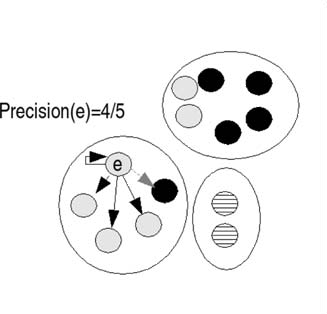
\includegraphics[width=0.2\linewidth, valign=c]{C:/Users/langh/Active Learning/Critical Analysis Essays/Effective-and-Generalizable-Graph-Based-Clustering-for-Faces-in-the-Wild/images/A Comparison of Extrinsic Clustering Evaluation Metrics/precision.png}
\]

\[
\text{BCubed-Recall} = Avg_e\left[\frac{\sum_{L(e)=L(e')}{\text{Correctness(e,e')}}}{\sum_{L(e)=L(e')}{1}}\right] \qquad 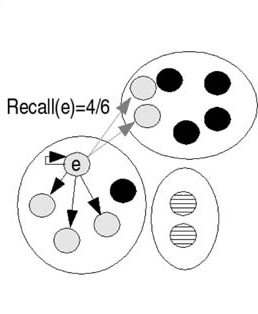
\includegraphics[width=0.2\linewidth, valign=c]{C:/Users/langh/Active Learning/Critical Analysis Essays/Effective-and-Generalizable-Graph-Based-Clustering-for-Faces-in-the-Wild/images/A Comparison of Extrinsic Clustering Evaluation Metrics/recall.png}
\]
\normalsize

\begin{figure}
\centering
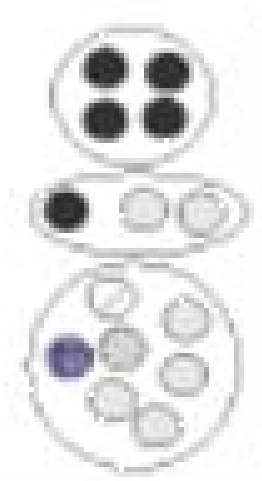
\includegraphics[height=2 in]{C:/Users/langh/Active Learning/Critical Analysis Essays/Effective-and-Generalizable-Graph-Based-Clustering-for-Faces-in-the-Wild/images/A Comparison of Extrinsic Clustering Evaluation Metrics/bcubed.png}
\caption{BCubed clustering example.\label{fig:bcubed}}
\end{figure}

Equation \ref{eq:bcubed-fmeasure} shows the BCubed FMeasure for clusters shown in Figure \ref{fig:bcubed}.

\small

\begin{equation}
\begin{aligned}
\text{BCubed-Precision} &= \frac{\textcolor{red}{4}*\frac{\textcolor{red}{4}}{4}+\textcolor{red}{1}*\frac{\textcolor{red}{1}}{3}+\textcolor{red}{2}*\frac{\textcolor{red}{2}}{3}+\textcolor{red}{1}*\frac{\textcolor{red}{1}}{7}+\textcolor{red}{1}*\frac{\textcolor{red}{1}}{7}+\textcolor{red}{1}*\frac{\textcolor{red}{1}}{7}+\textcolor{red}{4}*\frac{\textcolor{red}{4}}{7}}{14} \\
& = \textcolor{blue}{0.5986394557823128}\\
\text{BCubed-Recall} &= \frac{\textcolor{red}{4}*\frac{\textcolor{red}{4}}{5}+\textcolor{red}{1}*\frac{\textcolor{red}{1}}{5}+\textcolor{red}{2}*\frac{\textcolor{red}{2}}{6}+\textcolor{red}{1}*\frac{\textcolor{red}{1}}{1}+\textcolor{red}{1}*\frac{\textcolor{red}{1}}{1}+\textcolor{red}{1}*\frac{\textcolor{red}{1}}{1}+\textcolor{red}{4}*\frac{\textcolor{red}{4}}{6}}{14} \\
& = \textcolor{blue}{0.6952380952380952}\\
\text{BCubed-FMeasure} &= 2\cdot\frac{0.5986394557823128\cdot0.6952380952380952}{0.5986394557823128+0.6952380952380952}\\
& = \textcolor{blue}{0.6433328326072805}
\end{aligned}
\label{eq:bcubed-fmeasure}\end{equation}
\normalsize

Second, the threshold is evaluated independently using a range of combinations that cover values around the one that produced the most performance. The authors present the best results from values between 0.25 and 0.55 in steps of 0.05. A single value of 0.40 was found to be the best among the four datasets.

Finally, computation time is shown for each of the approaches and datasets with the best threshold for each. The authors fixed the face descriptor to ResNet-29 to isolate the performance of the clustering algorithm from confounders. Significant improvements were found in the YTF dataset in contrast to the Approximate Rank-order approach.

\hypertarget{contribution}{%
\subsubsection{Contribution}\label{contribution}}

The main contribution of this paper is that it proposes to add 2 post processing steps to the CW graph clustering approach to reduce the number of clusters found. The paper is mainly presented as an extension of the results obtained by \autocite{otto2018} using Approximate Rank-order.

A second contribution is the introduction of the BCubed metric in the evaluation protocol for face clustering. The BCubed metric meets the four constraints proposed in \autocite{amigo2009} and weights clusters linearly based on their size advantage. See Figure \ref{fig:conditions} for a depiction of these constraints.

\begin{figure}
\centering
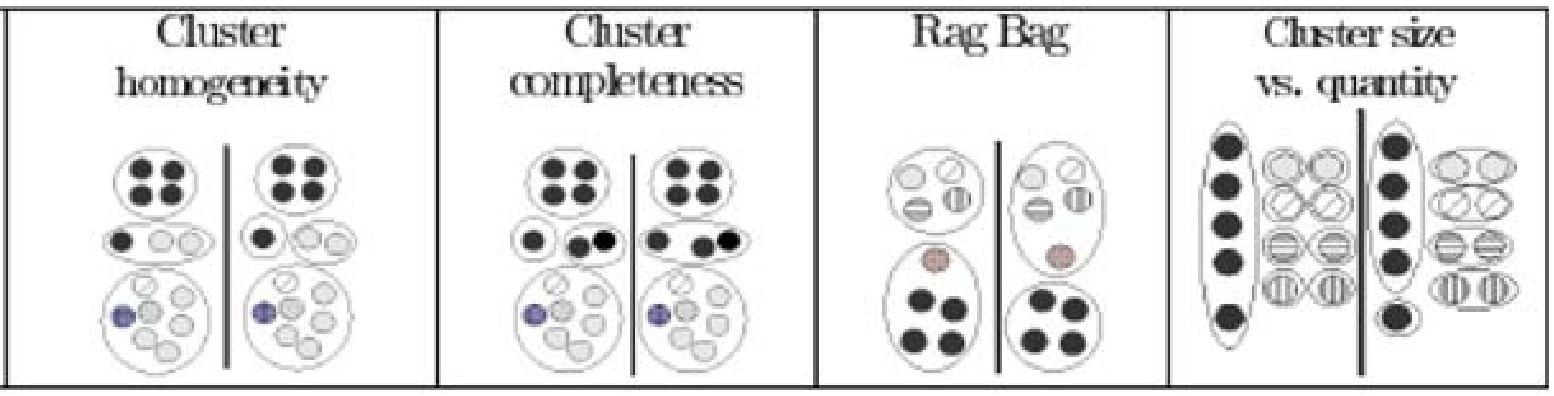
\includegraphics[width=1\linewidth]{C:/Users/langh/Active Learning/Critical Analysis Essays/Effective-and-Generalizable-Graph-Based-Clustering-for-Faces-in-the-Wild/images/A Comparison of Extrinsic Clustering Evaluation Metrics/conditions.png}
\caption{The four constraints proposed by \autocite{amigo2009}.\label{fig:conditions}}
\end{figure}

A third contribution of the paper is that the approach depends on finetuning only two parameters: (1) number of iterations for the CW algorithm and (2) the threshold for building a higher level of cluster abstraction and reapply CW. Of the two parameters, higher values for the former lead the algorithm to converge, so just selecting a high value here will do. For the latter, the authors present the best results from values between 0.25 and 0.55 in steps of 0.05.

Finally, the authors found a single threshold value that performs best for all the datasets under the current face representation. This is a great advantage over previous approaches because in real world scenarios there is no training data to finetune any parameter. By contrast, the paper by \autocite{otto2018} depends on finetuning its several parameters for the particular scenario.

\hypertarget{weaknesses}{%
\subsubsection{Weaknesses}\label{weaknesses}}

Face embeddings are extracted using a 29-ResNet. Samples for training this primal network are assumed to be independent and identically distributed as the samples from the other 4 datasets. The independence assumption might hold but the primal sample distribution might be in fact biased towards one of the following 4 testing datasets.

Also, the authors hint that some datasets have a great number of outliers, i.e.~subjects that have less than two instances. Conclusions derived from the results using such imbalanced datasets must take this fact into account or opt to filter those cases out.

Finally, the authors affirm that the single manually found threshold is scalable to other datasets. However, this threshold is bound to the specific 128D vector representation and probably even to the ResNet architecture. There is no evidence that the aforementioned representation generalize equally well to all datasets in the real world. Thus, this assertion is more general than it should.

\hypertarget{future-work}{%
\subsubsection{Future Work}\label{future-work}}

Chang points out the necessity to enforce pairwise constraints, i.e.~must-link and cannot-link relations to improve face clustering accuracy in scenes containing multiple faces, as proposed by \autocite{otto2018}.

\begin{figure}
\centering
\begin{tabular}{cc}
\subfloat[Must-link constraint]{
\includegraphics[width = 0.45\linewidth]{{"C:/Users/langh/Active Learning/Critical Analysis Essays/Effective-and-Generalizable-Graph-Based-Clustering-for-Faces-in-the-Wild/images/Constrained Multi-View Video Face Clustering/041"}.jpg}
} &
\subfloat[Cannot-link constraint]{
\includegraphics[width = 0.45\linewidth]{{"C:/Users/langh/Active Learning/Critical Analysis Essays/Effective-and-Generalizable-Graph-Based-Clustering-for-Faces-in-the-Wild/images/Constrained Multi-View Video Face Clustering/043"}.jpg}
}
\end{tabular}
\caption[Caption LOF]{Pairwise contraints from \autocite{wu2013}}
\end{figure}

\printbibliography


\end{document}
